\chapter{Development of Balance System}

\section{Development of module through OOP, managing models and controllers}

As discused before, the core elements composing a store's balance system are Balance Updates and Bank Transfers. These elements are constructed as Models, which in terms of OOP are represented by Classes. These Classes' attributes and elements will be handled independently by Models and Controllers Classes. Every action or method regarding the models will be handled by the Controllers.\\

The Controllers will generate instances of the Balance Updates and Bank Transfers models and handle the relationships between them. They will serve as the link between the application and the Database as well by using TypeORM Repositories for these Models.

\subsection{Balance Updates}

The System's general balance will be composed by numerous Balance Updates. Where the changes in the balance of the store will be reflected on each of them. As shown in Figure \ref{fig:uml_balance_update}, every instance will have its own \textit{id} as primary key, which will serve as reference for any foreign key relationship. The atribute \textit{amount} indicates exactly how the store's balance will be updated, by keeping a record of the store's previous balance and the current balance after the update was added in the respective attributes.

\begin{figure} [H]
    \centering
    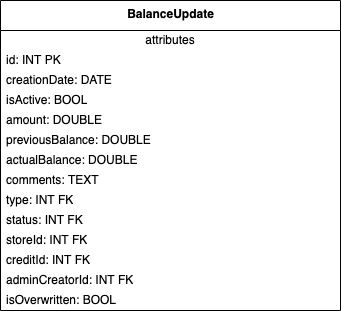
\includegraphics[scale = 0.7]{assets/uml/BalanceUpdate.png}
    \caption{Balance Update UML}\label{fig:uml_balance_update}
\end{figure}

Every Balance Update must have a \textit{storeId} foreign key, indicating which store's balance it is affecting. 

The attribute \textit{creditId} will serve as a reference for linking a credit entity to the Balance Update it created when it served as a \textit{Contribution} or \textit{Credit cancelation} to the store's balance. These refere to the types that a Balance Update could have and will be furtherly explained in section the following section. 

Some Balance Updates could be manually generated by any administrator with the appropiate permissions. For this scenario, it is important to keep a record of who made these changes by saving this administrator's id in the attribute \textit{adminCreatorId} and label these changes with the respective \textit{type}. 


\subsubsection{Balance Updates Types}

Every Balance Update will have a specific \textit{type} attribute. These types are managed as a table with static values and referenced through their \textit{id} attribute. A Balance Update could have specific behaviours depending on the status it has. For this reason, the type can not be edited once the instance of the Balance Update is generated. The different possible types of Balance Updates are described in Figure \ref{fig:balance_updates_types} 

\begin{figure}[ht]
    \caption{Balance Update Types}\label{fig:balance_updates_types}
    \begin{tabularx}{0.9\textwidth} { 
    | >{\centering\arraybackslash}X 
    | >{\centering\arraybackslash}X 
    | >{\raggedright\arraybackslash}X | }
   \hline
   id & Type & Description \\
   \hline
   1 & \textit{Contribution} & Contribution to balance due to a new credit   \\
   \hline
   1 & \textit{Disbursement} & Disbursement generated through the confirmation of a Bank Transfer   \\
   \hline
   1 & \textit{Credit Cancelation} & Loads negative balance due to credit cancelation   \\
   \hline
   1 & \textit{Adjustment} & Loads adjustment in balance to be considered in the next Bank Transfer   \\
   \hline
   1 & \textit{Disbursement override} & Overrides the amount addedd to the balance from another Disbursement   \\
   \hline
   1 & \textit{Balance compensation} & Readjusts the balance of a store by taking previous pending balance to apply immeditaly a credit's contribution   \\
   \hline
   1 & \textit{Balance readjustment} & Readjusts the balance of a store by updating Pending Balance Updates into Applied   \\
  \hline
\end{tabularx}
\end{figure}

\subsubsection{Balance Updates Status}

\begin{figure} [!htb]
    \centering
    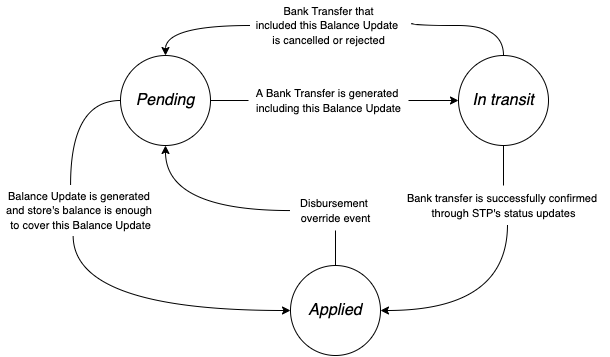
\includegraphics[scale = 0.7]{assets/diagrams/BalanceUpdatesStateMachine.png}
    \caption{Balance Updates State Machine}\label{fig:state_machine_balance_updates}
\end{figure}


\subsubsection{Overwriting Balance Updates}


Balance Updates have an attribute to indicate if the object was overwritten. Whenever an object is overwritten, this means that there is an additional Balance Update that is cancelling its affectation on the store’s general balance. This is particularly helpful to keep control of a store’s balance modification for those Balance Updates that are generated with the status of Applied. The only Balance Updates that could be overwritten are those of the types of Disbursement and Contribution.\\

A Balance Update of type Disbursement is generated whenever a confirmation that a Bank Transfer has been successfully accepted by the receiving party is received. There is a very particular edge case where the money could be returned even after it was confirmed. For these cases, the Disbursement that was generated is no longer valid, hence, an update to the store’s balance should be made. This is done by generating an additional Balance Update with type Disbursement Override. This new Balance Update will contribute once again the amount that was marked as disbursed to the store’s balance.\\

Furthermore, Balance Updates of type Contribution could also be overwritten at some point. These are created once a partner has confirmed a product’s delivery through their dashboard and the credit of that product will generate a contribution to the store’s balance. This means that there is some amount that Atrato must eventually transfer to the partner’s bank account depending on the disbursement modality that this partner has active. These contributions could eventually be overwritten if the credit is later cancelled, which may happen at some points for external reasons. For this particular scenario, a new Balance Update of type Credit cancelation needs to be created to compensate the previous contribution, regardless of the contribution’s status as shown in Figure \ref{fig:dlowchart_credit_cancelation}.

\begin{figure} [h]
    \centering
    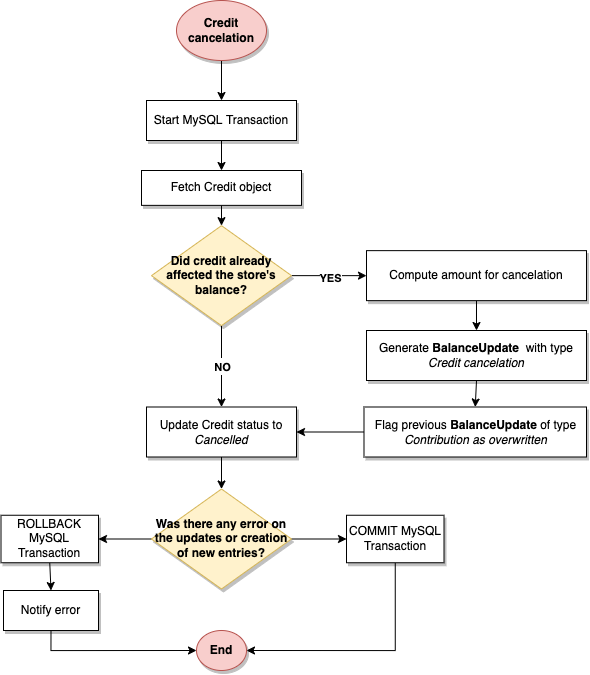
\includegraphics[scale = 0.7]{assets/flowcharts/CreditCancelation.png}
    \caption{Processing a credit's cancelation and its affectation to a store's balance system}\label{fig:dlowchart_credit_cancelation}
\end{figure}

\section{Ensure correct functionality and error handling through MySQL Transactions}

\section{Detailed visibility and traceability of full process}

\subsection{Implementation of existing Logging system}

\section{Security through implementation of existing IAM Module}

\section{Manual implementation of automation}
